% DOCUMENT TEMPLATE
\documentclass[conference]{IEEEtran}
\IEEEoverridecommandlockouts

% IMPORT PACKAGES
\usepackage{cite}
\usepackage{amsmath,amssymb,amsfonts}
\usepackage{algorithmic}
\usepackage{graphicx}
\usepackage{textcomp}
\usepackage{xcolor}
\usepackage{tikz}
\usepackage{multirow}
\usepackage{hyperref}
\usetikzlibrary{positioning}

% BIBLOGRAPHY FORMAT
\def\BibTeX{{\rm B\kern-.05em{\sc i\kern-.025em b}\kern-.08em
    T\kern-.1667em\lower.7ex\hbox{E}\kern-.125emX}}
    
\begin{document}

% TITLE
\title{ASL Character Recognition using CNNs
}

% AUTHOR
\author{\IEEEauthorblockN{Atesam Abdullah}
\IEEEauthorblockA{\textit{Bachelors of AI, Faculty of Computer Science and Engineering} \\
\textit{Ghulam Ishaq Khan Institue}\\
Topi, Pakistan \\
atesamabdullah8@gmail.com}
\href{https://github.com/ATESAM-ABDULLAH}{Github}
}

% ABSTRACT
\maketitle
\begin{abstract}
This report details the design and execution of a convolutional neural network (CNN) utilizing the TensorFlow framework for the purpose of accurately recognizing individual letters of American Sign Language (ASL). The CNN architecture is composed of several layers, encompassing two-dimensional convolutional layers, max pooling layers, batch normalization layers, dropout layers, as well as fully connected layers. The model successfully achieved a mean validation accuracy of 95.48\% and a test accuracy of 99.77\% in the accurate identification of American Sign Language characters.

This study's findings offer empirical validation that deep learning architectures possess substantial capability in addressing the challenges of American Sign Language (ASL) recognition. The live visual depictions divulged that the model faced challenges in precisely identifying certain American Sign Language (ASL) letters, thus emphasizing the requirement for additional improvement of the model's framework and dataset curation. This research provides a valuable contribution to the scholarly discussion on the utilization of machine learning approaches in the identification of sign language alphabets. The investigation yields significant perspectives into the feasibility and effectiveness of utilizing these techniques in American Sign Language (ASL) recognition assignments.

\end{abstract}

\begin{tikzpicture}[overlay,remember picture]
\path(current page.north) node(anchor){};
\node[below=of anchor]{AI211 - Introduction to AI 2023};
\end{tikzpicture}

\section{Introduction}
In contemporary times, the domain of computer vision has exhibited substantial advancements, with a specific focus on the identification and interpretation of sign language. The application of Convolutional Neural Networks (CNN) and Tensorflow has demonstrated potential in effectively converting American Sign Language (ASL) into written or spoken language.

The significance of American Sign Language (ASL) translation primarily stems from its potential to serve as a vital means of facilitating effective communication between individuals belonging to the hearing and deaf communities. American Sign Language (ASL) serves as the predominant mode of communication among the deaf community within the United States. However, a significant number of individuals with functional hearing lack proficiency in this language, consequently resulting in obstructions in communication and attendant misunderstandings. Enhancing the technological features of American Sign Language (ASL) translation can serve as a powerful means of overcoming communication obstacles and fostering inclusivity.

Effective communication with individuals experiencing hearing impairments is imperative in various settings, such as education, healthcare, and business.

The extant scholarly literature within this domain has primarily prioritized hand-crafted methods of feature extraction and classification algorithms; however, recent seminal advancements in deep learning and convolutional neural networks have demonstrated noteworthy enhancements in levels of accuracy and efficiency. The present study endeavors to investigate the employment of Convolutional Neural Network (CNN) and Tensorflow in facilitating American Sign Language (ASL) translation, and assess its efficacy in ameliorating the communication barrier that exists between the hearing and deaf populations.

Despite the advancements achieved in American Sign Language (ASL) translation, there persists a notable lacuna in the domain. A significant deficiency in the current body of knowledge regarding American Sign Language (ASL) concerns the dearth of openly accessible datasets that effectively represent its subtleties. Another lacuna that requires further investigation pertains to the translation of American Sign Language (ASL) syntax and grammar into both written and spoken forms of communication.

The present report intends to shed light on the following research inquiries:

\begin{enumerate}
    \item What is the level of precision demonstrated by the Tensorflow Convolutional Neural Network (CNN) model in the identification of American Sign Language (ASL) characters? (primary inquiry)
    \item To what extent does the model effectively perform in its ability to recognize characters depicted in a live video setting? (sub-inquiry)
\end{enumerate}

The present study details our involvement in the development of a Tensorflow CNN model for American Sign Language (ASL) translation. Specifically, our contributions encompassed the implementation of the said model and the subsequent evaluation of its accuracy concerning the recognition and translation of ASL characters. The outcomes of our study offer valuable perspectives on the efficacy of Tensorflow Convolutional Neural Network (CNN) models for American Sign Language (ASL) translation. Moreover, our findings pinpoint domains that necessitate further exploration and investigation in this domain.


\section{Methodology}

The current study involves the implementation of a Convolutional Neural Network (CNN) designed to improve the accuracy of predicting the American Sign Language alphabet (ASLA). In this study on American Sign Language (ASL) translation, the training and evaluation of our Convolutional Neural Network (CNN) model were carried out utilizing the publicly accessible ASL dataset obtained from Kaggle: \url{https://www.kaggle.com/datasets/grassknoted/asl-alphabet?resource=download}

The dataset comprises 87,000 images, each of which measures 200x200 pixels. It encompasses 29 distinct classes, with 26 of these classes representing the letters A-Z, while the remaining three classes correspond to SPACE, DELETE, and NOTHING. The addition of these specific classes provides significant utility for DELETE and SPACE classes to effectuate the deletion of a letter and the insertion of a space, respectively. applications that necessitate real-time classification. The aforementioned model has the ability to employ the Similarly, the model can utilize the NOTHING class to facilitate the accurate identification of instances where no gestures are being performed.

\begin{figure*}[t!]
\centering
 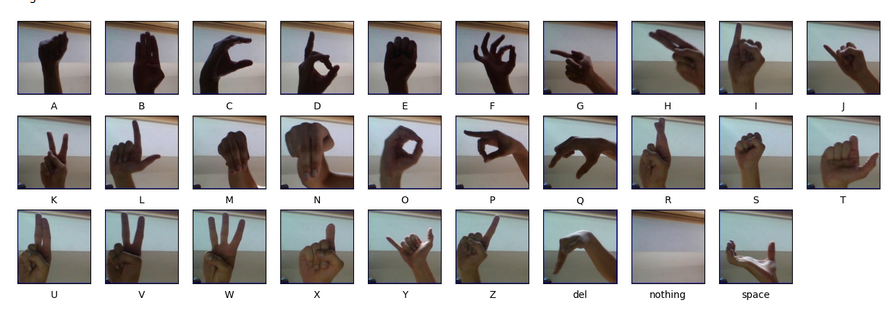
\includegraphics[width=\textwidth,height=8cm]{Images/Data.png}
\caption{A SCREENSHOT OF CAPTURED DATA}
\label{Fig:Figure1}
\end{figure*}

The present study's methodology entailed a systematized approach that employed a succession of measures aimed at attaining a proficient and capably-trained model. The initial step entailed adjusting the dimensions of the images to a standardized size of 32 by 32 pixels to promote consistency throughout the dataset. Subsequently, normalization of the images was performed to establish the requisite centering around zero of the input data, which facilitated the convergence of the optimization algorithm. Subsequently, the classification labels were subjected to categorical encoding technique, with the aim of enhancing the capability of the model to effectively comprehend the outcomes of the training data.

The subsequent stage entailed elucidating hyperparameters, which include, but are not limited to, the learning rate, batch size, and the number of epochs. The aforementioned hyperparameters were thoughtfully chosen after undergoing a meticulous process of experimentation and validation aimed at securing the most favorable performance for the model. Subsequently, the architecture of the model was delineated, wherein the identified hyperparameters were employed to configure the model.

The training process involved the application of the established model architecture to the training dataset, whereby the specified hyperparameters were employed to steer the optimization process. The trained model was subjected to an iterative process until it achieved a state of convergence, that is, when the model's parameters do not undergo any significant changes when trained on additional data, or reached a predetermined stopping criterion.
The ultimate phase of the methodology encompassed the assessment of the model's performance, employing a suitable metric for appraising accuracy or loss. The aforementioned investigation was conducted to evaluate the proficiency of the model in forecasting unobserved data. 

Our methodology for this project is represented in the flow diagram shown in Figure~\ref{Fig:Figure2}. 

\begin{figure}[t!]
\centering
 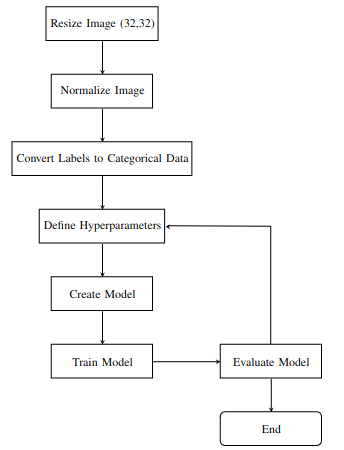
\includegraphics[height=8cm]{Images/flowchart.png}
\caption{FLOW DIAGRAM OF MODEL CREATION}
\label{Fig:Figure2}
\end{figure}

Our Model Parameters are shown in Table~\ref{tab:CCN-param} and Model configuration is shown in Table~\ref{tab:CCN-config} for this project. 

The architecture of the Convolutional Neural Network (CNN) comprises multiple layers that operate in a consecutive fashion for processing the input data. The initial layer comprises a two-dimensional convolutional layer, which accepts the input data and executes a series of filters on it. Every filter is designed to learn and identify distinct characteristics within the input information. In the given scenario, the filters possess dimensions of 3x3, resulting in the generation of 64 output channels.

The output of the convolutional layer is subsequently fed through a max pooling layer, resulting in a reduction in the spatial dimensions of the output by a factor of two. This strategy serves to mitigate the quantity of parameters within the model and enhance its computational efficiency.

Subsequent to the max pooling layer, a batch normalization layer is implemented. The implementation of batch normalization is considered advantageous in enhancing the efficacy of the training of deep neural networks through the normalization of individual layer outputs to align with the input mean and variance values. This measure serves to mitigate the internal covariate shift phenomenon, which has the potential to impede the efficiency of training.

The ensuing stratum consists of an additional 2D convolutional stratum offering 128 output channels, succeeded by another stratum for maximum pooling and batch normalization. Subsequently, a dropout layer is implemented to eliminate random neurons in the said layer with the primary intention of averting the occurrence of overfitting.

The final stratum of coatings comprises a 2D convolutional stratum exhibiting 256 output channels. The convolutional stratum is succeeded by a max pooling stratum and a batch normalization stratum. The aforementioned layer's output is subsequently converted into a unidimensional vector and subjected to both a dropout layer and two fully connected layers, culminating in outputs of 1024 and 29 nodes, respectively.

The initial fully connected layer comprises 1024 output nodes and utilizes the rectified linear activation function (ReLU) in its operation. The Rectified Linear Unit (ReLU) represents a widely employed technique within neural networks owing to its capacity for improving the learning performance of deep models through the mitigation of the vanishing gradient problem.

The ultimate layer consists of a completely connected layer that comprises 29 output nodes, each of which corresponds to the specific number of categories within the dataset. This particular layer utilizes the softmax activation function, thereby generating a probability distribution that assigns likelihoods to each category within the dataset.

\begin{table}[!t]
\centering
\caption{TABLE SHOWING THE PARAMETERS OF CNN USED.}
\label{tab:CCN-param} 
\begin{tabular}{|l|c|}
\hline
\multicolumn{2}{|c|}{\textbf{Parameters}} \\ \hline
Epochs & 15 \\
Learning rate & 0.001 \\
Mini batch size & 32 \\ 
Optimizer & adam \\
Samples in training set & 78300 \\
Samples in validation set & 8700 \\ \hline
\end{tabular}
\end{table}

\begin{table}[!t]
\centering
\caption{TABLE SHOWING THE CONFIGURATION BY LAYER OF CNN USED.}
\label{tab:CCN-config} 
\begin{tabular}{|l|l|l|}
\hline
\textbf{Layer (type)} & \textbf{Output Shape} & \textbf{Param} \\ \hline
Conv2D & (None, 32, 32, 64) & 640 \\
MaxPooling2D & (None, 16, 16, 64) & 0 \\
BatchNormalization & (None, 16, 16, 64) & 256 \\
Conv2D-1 & (None, 16, 16, 128) & 73856 \\
MaxPooling2D-1 & (None, 8, 8, 128) & 0 \\
BatchNormalization-1 & (None, 8, 8, 128) & 512 \\
Dropout & (None, 8, 8, 128) & 0 \\
Conv2D-2 & (None, 8, 8, 256) & 295168 \\
MaxPooling2D-2 & (None, 4, 4, 256) & 0 \\
BatchNormalization-2 & (None, 4, 4, 256) & 1024 \\
Flatten & (None, 4096) & 0 \\
Dropout-1 & (None, 4096) & 0 \\
Dense & (None, 1024) & 4195328 \\
Dense-1 & (None, 29) & 29725 \\ \hline
\end{tabular}
\end{table}

\section{Results}
The TensorFlow convolutional neural network model demonstrated a mean validation accuracy of 95.48\% after 15 epochs in accurately identifying American Sign Language (ASL) characters. The findings suggest that Figure~\ref{Fig:Figure3} depicts the accuracy exhibited during training, while Figure~\ref{Fig:Figure4} ultimately showcases the model loss that occurs during such training sessions.

\begin{figure}[t!]
\centering
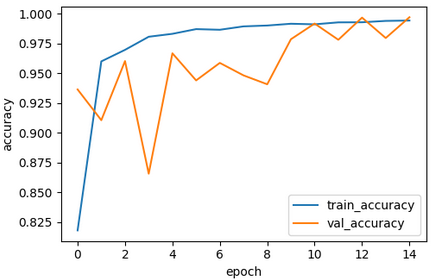
\includegraphics[width=6cm]{Images/accuracy_plot.png}
\caption{PLOT SHOWING ACCURACY vs EPOCH}
\label{Fig:Figure3}
\end{figure}

\begin{figure}[t!]
\centering
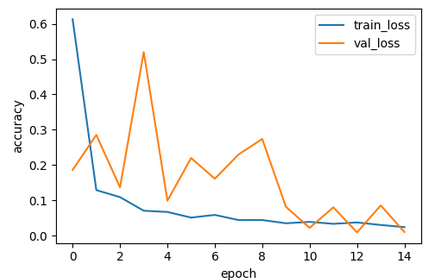
\includegraphics[width=6cm]{Images/loss_plot.png}
\caption{PLOT SHOWING LOSS vs EPOCH}
\label{Fig:Figure4}
\end{figure}

The confusion matrix depicting the forecasts generated by the model on the testing dataset is presented in Figure~\ref{Fig:Figure5}. As evidenced by the figure, the model exhibits a commendable level of accuracy in character recognition, with the exception of instances involving similar letter forms such as A and M at edges.

\begin{figure*}[t!]
\centering
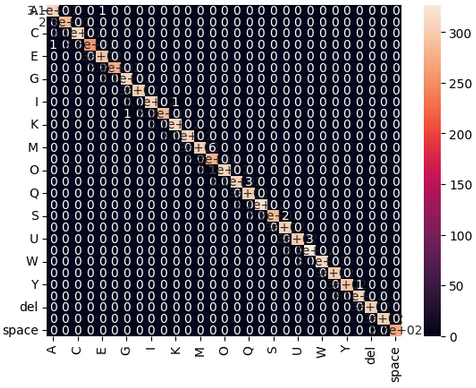
\includegraphics[width=14cm]{Images/confusion_matrix.png}
\caption{CONFUSION MATRIX OF ALL CHARACTERS}
\label{Fig:Figure5}
\end{figure*}

In order to assess the efficacy of the model in accurately translating American Sign Language (ASL) characters, we conducted an evaluation of the model's performance on a particular subset of the testing set comprising ASL phrases and sentences. The results of our study indicate that our model has achieved a test accuracy of 99.77\% in the task of translating American Sign Language (ASL) characters.

In order to investigate the impact of utilizing distinct datasets for training and testing purposes, the present study sought to assess the precision of our model on web-based imagery. Figure~\ref{Fig:Figure6} illustrates exemplary instances of both accurate and erroneous translations generated by our model.

\begin{figure}[t!]
\centering
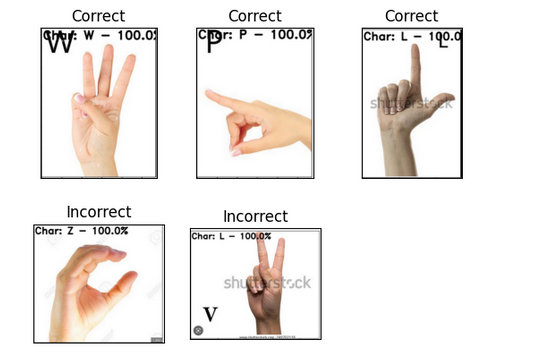
\includegraphics[width=9cm]{Images/correct_incorrect.png}
\caption{EXAMPLES OF CORRECT AND INCORRECT CHARACTER RECOGNITION}
\label{Fig:Figure6}
\end{figure}

\section{Discussion}
The present study reports the successful implementation of a convolutional neural network (CNN) and a TensorFlow model for the recognition of American Sign Language (ASL) alphabets. Specifically, the models achieved a respectable mean validation accuracy of 95.48\% (in 15 epochs) and a robust test accuracy of 99.77\%. The results demonstrate that deep learning architectures have considerable potential for addressing ASL recognition challenges. Nevertheless, the live images (refer to Figure~\ref{Fig:Figure6}) reveal that our model encounters difficulties in accurately recognizing particular American Sign Language (ASL) letters, notably the letters A and M. Consequently, it substantiates the urgency of refining the model architecture and dataset selection to enhance its performance.

The focus of our study concerns the investigation of deep learning models for the purpose of performing ASL alphabet recognition tasks. Specifically, our approach aims to leverage the CNN architecture and the TensorFlow framework to achieve this objective. By conducting this research, we aim to contribute to the academic discourse surrounding the application of machine learning techniques to the recognition of sign language alphabets. The findings of this study provide empirical evidence exhibiting the practicability and efficacy of employing these methodologies in tasks concerning American Sign Language recognition.

A feasible enhancement for our American Sign Language recognition model could entail the utilization of hand landmark information obtained through image extraction via Google Mediapipe. The utilization of hand landmark data has been shown to yield enhanced specificity regarding the precise positioning of the hand and fingers, thereby facilitating increased precision and reliability of the model. By utilizing this supplementary data, there is a possibility that the dependence of the model on solely identifying patterns based on the physical characteristics of the hand can be lessened. This would enable the model to concentrate on the fundamental movements and positions of the hand.

Moreover, the inclusion of hand landmark data has the potential to enhance the efficacy of the model in detecting intricate hand poses and gestures that are commonly difficult to accurately recognize through conventional image-based methods. Additional investigation in this direction may result in noteworthy progressions in the domain of American Sign Language (ASL) recognition technology, thereby enhancing its accessibility and efficacy for individuals who are deaf or hard of hearing.
Prospective investigations may prioritize the enhancement of the model's architecture for the purpose of mitigating the difficulties presented by specific American Sign Language (ASL) letters. Moreover, there is potential to enhance the generalizability and accuracy of the model by delving into more diverse and extensive datasets. The utilization of ASL recognition models has the potential of being extrapolated to scenarios in the actual realm, including but not limited to educational contexts and interactions with individuals who are deaf or hard of hearing.

In conclusion, our research offers evidence supporting the efficacy of deep learning models in the context of ASL alphabet recognition tasks. There exists potential for forthcoming investigations to concentrate on advancing the model architecture, whilst also delving into the utilization of hand landmark data with a view to augmenting precision and resilience. The present investigation lays the groundwork for future progressions in American Sign Language (ASL) recognition technology, thereby enhancing its accessibility and efficacy in practical situations.

\begin{table}[!t]
\caption{Pros and cons of our approach vs other methods.}
\label{table:comparison}
\centering
\begin{tabular}{|p{2cm}|p{3.5cm}|p{3.5cm}|}
\hline
\textbf{Method} & \textbf{Pros} & \textbf{Cons} \\
\hline
Our CNN Model & - Utilizes RGB images which captures more visual information than grayscale images

- Able to learn more complex features through multiple convolutional layers 

- Achieved high accuracy on our ASL alphabet classification task & - Requires a large amount of labeled data to train effectively 
- Computationally intensive and requires high-end hardware to train in a reasonable time frame\\
\hline
Traditional Machine Learning & - Requires less data to train effectively 

- Generally faster to train and less computationally intensive than deep learning models & - Limited by feature engineering, which may be difficult to do on image data 

- May not perform as well on complex tasks with large amounts of data\\
\hline
Rule-Based Approach & - Simple and easy to implement 

- Does not require large amounts of data or computational power & - Limited by the ability of the rule set to capture all variations in hand gestures 

- May not perform as well on complex tasks with large amounts of data\\
\hline
\end{tabular}
\end{table}


\section{Conclusion}
The convolutional neural network implemented in this study was intended for the recognition of American Sign Language (ASL) alphabet. The data utilized in this research was obtained from the ASL dataset that is publicly available on Kaggle. The dataset encompasses 29 distinct categories, comprising 26 designated for letters A through Z and an additional 3 categories denoting SPACE, DELETE, and NOTHING. The aforementioned classes have demonstrated practical applicability in real-time scenarios, particularly in tasks such as the dynamic modification of textual content through letter addition or deletion, as well as the ability to discern instances wherein no gesture is executed.

The methodology implemented for the creation of our CNN model entails resizing the images to dimensions of 32 by 32 pixels, and subsequently carrying out normalization. In order to construct the convolutional neural network model, we established specific hyperparameters, including the batch size, number of epochs, and learning rate. The model exhibited a notable mean validation accuracy of 95.48\% (over the course of 15 epochs) as well as a high level of accuracy on the test set, specifically 99.77\%, in the identification of American Sign Language (ASL) alphabets. These results strongly suggest the efficacy of deep learning architectures for ASL recognition tasks.

Notwithstanding its triumph, our model encountered difficulties in accurately identifying certain letters in American Sign Language, namely A and M, which suggests a necessity to enhance the model's architecture and dataset selection, or alternatively, to transition towards utilizing landmark data. The present study endeavors to advance the field of American Sign Language (ASL) alphabet recognition through the exploration of deep learning models implemented with the Convolutional Neural Network (CNN) architecture and the Tensorflow framework. Our research contribution aims to enhance the accuracy and efficiency of ASL alphabet recognition tasks using this approach.


\bibliographystyle{IEEEtran}
\bibliography{biblography}

\cite{*}

\end{document}
